\noindent

\subsection{Reviewer-reviewer interaction network}
\label{rev_int_net} 
The reviewer-reviewer interaction network is created with each node representing a reviewer and an edge exists between two reviewers if they have been assigned by at least one common editor. We devote the rest of the section in demonstrating the importance of the various structural properties of the network in determining the long term citation of the paper. Note that there are 4035 unique reviewers in the system each of which form a node in this network.

\begin{figure*}
\centering
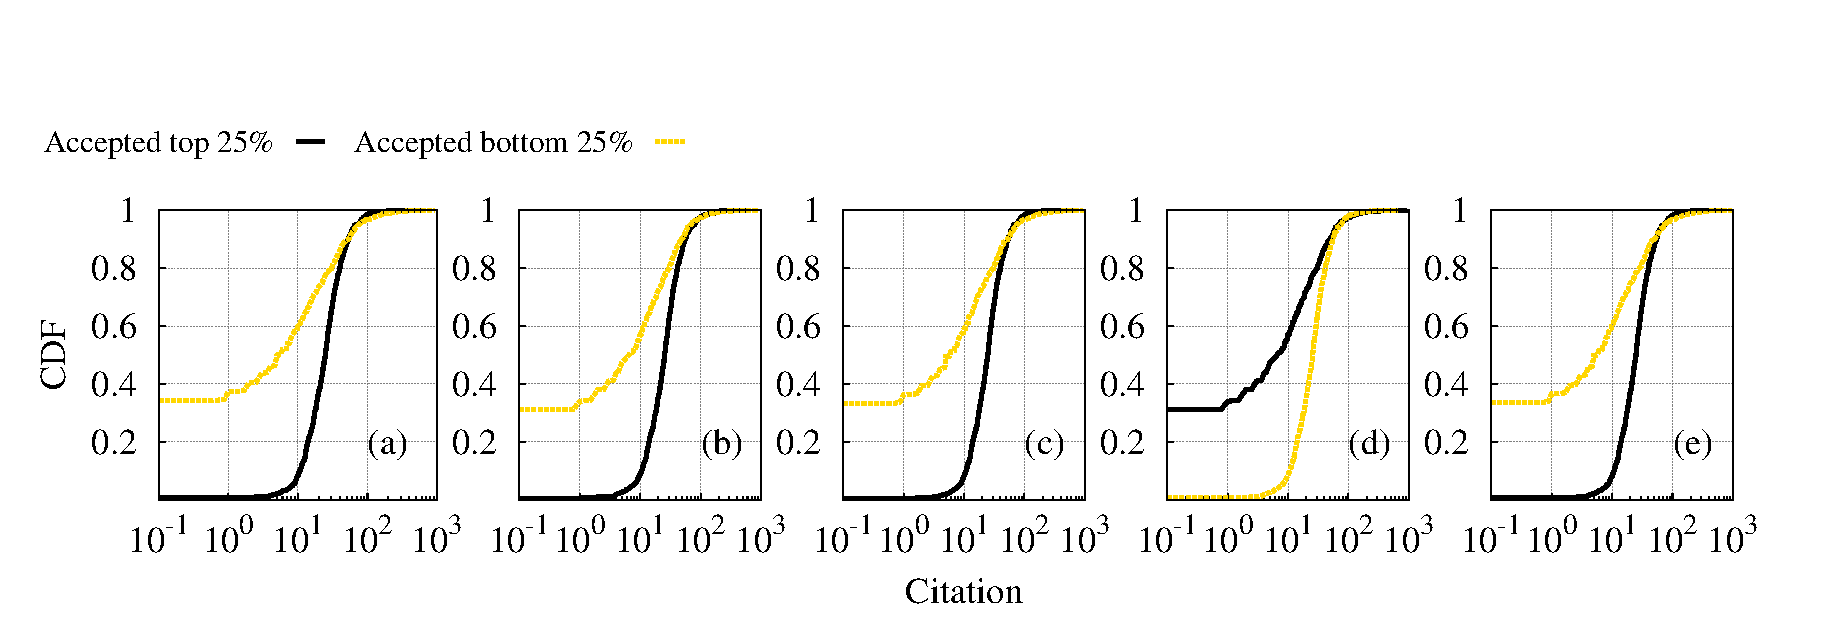
\includegraphics[width = 0.9\textwidth]{./texfiles/Chapter_4/jcdl/figures/citation_.eps} 
\caption{\label{fig:net_citation} Cumulative distribution function (CDF) of citations received by the papers (accepted) reviewed by referees in top 25\% and bottom 25\% reviewers ranked according to (a) degree, (b) betweenness centrality, (c) closeness centrality (d) clustering coefficient values and (e) PageRank in the reviewer-reviewer interaction network.\vspace{4mm}}
\end{figure*}

\subsubsection{Degree (Deg)}
Degree of a node $v$ is the number of other nodes it is connected to in the network. A node with a higher degree in the reviewer-reviewer interaction network would indicate (i) assignment from multiple editors, (ii) assignment from a reputed editor (with large number of assignments) which in turn would indicate the reputation of the reviewer. To verify our hypothesis, we rank the reviewers based on their degree in the network and calculate the mean citation of the papers reviewed by the reviewers in the top and the bottom 25\% of the rank list. We observe that  the papers reviewed by the top 25\% reviewers receive much higher citations than the those reviewed by the bottom 25\% reviewers (refer to figure~\ref{fig:net_citation}(a)).    

\subsubsection{Betweenness centrality (BC)}

Betweenness centrality of a node quantifies the position of a node based on the number of shortest paths the node is part of. For every  pair of nodes in the network there exists a shortest path between them. Betweenness centrality of a node ($v$) is the fraction of all such paths that pass through $v$. In the reviewer-reviewer interaction network, a high  centrality value would indicate assignment by multiple editors and that this node acts as a bridge between them. We again rank the reviewers based on the betweenness centrality values and calculate the average citation of the papers. We find that the papers accepted by the top 25\% reviewers tend to be cited more compared to those accepted by the bottom 25\% (refer to figure~\ref{fig:net_citation}(b)). 

\subsubsection{Closeness centrality (CC)}

Formally closeness centrality of a node in a network is the inverse of the sum of length of its shortest path to all other nodes in the network. Hence higher centrality value indicates that the node is more closer to all other nodes in the network. In the reviewer-reviewer interaction network, a reputed reviewer will be assigned by multiple reviewers and hence will be closer to the other reviewers in the network. This is represented in figure~\ref{fig:net_citation}(c), where we show that the papers accepted by top 25\% most central reviewers 
are cited more often compared to the bottom 25\% reviewers. 

\subsubsection{Clustering coefficient (Clus)}

Clustering coefficient of a node is measured as the fraction of connections among the neighbors of the node. For the reviewer-reviewer interaction network, every reviewer assigned by a common editor is connected to every other reviewer in the network. A reviewer assigned by many editors would actually act as a bridge between two cliques and hence would have a lower clustering coefficient value compared to a reviewer who is part of a single clique (always assigned by a single editor). This is further demonstrated in  figure~\ref{fig:net_citation}(d) where we observe that the papers accepted by reviewers having lower clustering coefficient tend to be cited more.

\subsubsection{PageRank (PR)}

PageRank is a link analysis based algorithm that calculates for each node its relative importance within 
the network. Specifically, PageRank outputs a probability distribution which is used as the likelihood of a random walker to end up in a specific node. We simulate PageRank on the reviewer-reviewer interaction 
network to obtain the relative importance of each node. Further analysis indicates that the papers accepted by the top 25\% reviewers (based on PageRank) are cited more often compared to those accepted by the bottom 25\% reviewers (refer to figure~\ref{fig:net_citation}(e)). 

The above results thus indicate that simple network properties of the reviewer-reviewer interaction network could be highly effective in predicting the long-term citation of the paper at the time of publishing. 
\medskip